\section{Quality Assurance}
\label{sec:fdsp-tpcelec-qa}

%%%%%%%%%%%%%%%%%%%%%%%%%%%%%%%%%%%
\subsection{Introduction}
\label{sec:fdsp-tpcelec-qa-introduction}

The \dword{ce} consortium is developing a \dword{qa} plan that is consistent
with the principles discussed in the Technical Coordination part of this 
\dword{tdr} (Volume 7 Chapter 9). %Commented out because it breaks the automatic build system %(\refch{tc}{vl:tc-QA}).
The goal of the \dword{qa} plan is to maximize the number of functioning
read-out channels in the detector that achieve the performance specifications
for the detector that have been discussed in Section~\ref{sec:fdsp-tpcelec-overview-design},
in particular in terms of noise. Minimizing the noise in the detector involves
considering all system aspects already during the design phase, and in this
respect the experience gained with the \dword{pdsp} prototype is extremely
valuable and has been used to inform the design changes in the detector 
components. The lessons learned during the construction of \dword{pdsp},
the commissioning of the detector and the initial data taking period have
already been discussed in Section~\ref{sec:fdsp-tpcelec-design}. Further
operation of \dword{pdsp} in 2019 will continue to inform the final design
of the detector components.

Apart from the number of channels the most important difference
between \dword{pdsp} and DUNE is the projected lifetime of the detector. This
is relevant because significant fraction of the detector components provided 
by the \dword{ce} consortium are installed inside the cryostat and cannot 
be accessed or repaired during the operational lifetime of the detector. The 
Graded Approach to \dword{qa} implies that particular care needs to applied
to the \dword{ce} components that are installed inside the cryostat.

A complete \dword{qa} plan starts with ensuring that the design of all
the detector components fulfills the specification criteria, considering
also system aspects, i.e. how the various detector components interact
among themselves and with the detector components provided by other 
consortia. We discuss the validation of the design in 
Section~\ref{sec:fdsp-tpcelec-qa-initial} and the facilities that we use
to investigate the interaction between different detector components
in Section~\ref{sec:fdsp-tpcelec-qa-facilities}. 

The other aspects of the \dword{qa} plan involve documenting the 
assembly and testing processes, storing and analyzing the information
collected during the \dword{qc} process, training and qualifying the
personnel from the consortium, monitoring the procurement of 
components from external vendors, and assessing whether the
\dword{qc} procedures are being applied in a uniform way across
the various sites involved in the detector construction, integration,
and installation. The plan of the \dword{ce} consortium involves
having multiple sites performing the same \dword{qc} procedures,
with the possibility of a significant turnaround in the personnel
performing these tasks. To avoid problems during the bulk of the
production phase we plan to emphasize the training and documentation
aspects of the \dword{qa} plan. Reference parts will be tested at
multiple sites to ensure that consistent results are produced. At
a single site the same parts will be tested repeatedly to ensure
that there are no changes in the response of the apparatus and
that new personnel involved in testing detector components is 
as proficient as more experienced personnel. All the data from
the \dword{qc} process will be stored in a common database and
the yields of the production will be centrally monitored and 
compared among different sites. The procedures that will be adopted
during the detector construction will evolve from the experience
gained with \dword{pdsp}. A first version of the testing procedures
will be put in place in 2019 and 2020, while the final design of
the detector components is being completed and new prototypes are
being tested. The \dword{qc} procedures will be then reviewed
during the Engineering Design Review that precedes the beginning
of the pre-production. Lessons learned during the pre-production
will be analyzed and a final and improved \dword{qc} process will be 
developed prior to the Production Readiness Review that triggers
the beginning of the production. During the production the results
of the \dword{qc} process will be reviewed at regular interval
in Production Progress Reviews. In case of problems, production
will be stopped and an analysis of the issues will be performed
and will result in changes to the procedures if necessary.

%%%%%%%%%%%%%%%%%%%%%%%%%%%%%%%%%%%
\subsection{Initial Design Validation}
\label{sec:fdsp-tpcelec-qa-initial}

As described in Section~\ref{sec:fdsp-tpcelec-design}, four \dwords{asic} 
are being developed for the DUNE far detector single-phase TPC readout 
(\dword{larasic}, \dword{coldadc}, \dword{coldata}, and \dword{cryo}). 
When a new prototype \dword{asic} is produced, the first tests of 
\dword{asic} functionality and performance are done by the groups 
responsible for the \dword{asic} design. These tests may use either 
packaged parts or dice mounted directly on a printed circuit board 
and wire bonded to the board.  The goal of these tests is to determine 
the extent to which the \dword{asic} functions as intended, both at room 
temperature and at liquid Nitrogen temperature.  For all chips these tests 
include exercising digital control logic and all modes of operation. Tests 
of \dword{fe} \dwords{asic} include measurements of the noise as a function 
of input capacitance, baseline recovery from large pulses, cross-talk, linearity, 
and dynamic range. Tests of \dwords{adc} include effective noise and 
differential and integral non-linearity. Tests of \dword{coldata} and \dword{cryo} 
include verification of both the control and high speed data output links with 
cables at least as long at the longest cables needed in the DUNE far detectors 
(currently estimated to be 27 meters). After the initial functionality
tests performed by the groups that have designed the \dwords{asic} further
tests will be performed by other independent groups and then the \dwords{asic}
will be mounted on \dwords{femb} such that noise measurements can be repeated
with real \dword{apa}s attached to the readout, including the investigation
of possible system issues generated by the interaction with different 
detector components.

%%%%%%%%%%%%%%%%%%%%%%%%%%%%%%%%%%%
\subsection{Integrated Test Facilities}
\label{sec:fdsp-tpcelec-qa-facilities}

%%%%%%%%%%%%%%%%%%
\subsubsection{ProtoDUNE-SP}
\label{sec:fdsp-tpcelec-qa-facilities-pdune}

\dword{pdsp} is designed as a full slice of the \dword{spmod} as close as 
possible to the final DUNE \single components. It contains six full-size 
DUNE \dwords{apa} instrumented with \num{20} \dwords{femb} each for a 
total readout channel count of \num{15360} digitized sense wires. Critically, 
the wires on each \dword{apa} are read out via a full \dword{ce} readout 
system, including a \dword{ce} flange and \dword{wiec} with five \dwords{wib} 
and one \dword{ptc}. Each combined \dword{apa} and \dword{ce} readout follows 
the grounding guidelines described in Section~\ref{sec:fdsp-tpcelec-design-grounding} 
to operate as a complete isolated readout unit.

\dword{pdsp} took beam data in the CERN Neutrino Platform in 2018 and will continue
to take cosmic data throughout 2019. As described in Section~\ref{sec:fdsp-tpcelec-overview-pdune}, 
the live channel count (99.7\%) and average noise levels on the collection and induction wires 
(ENC$<$600e$^-$ and 800$^-$, respectively) satisfy the DUNE \single requirements described 
in Section~\ref{sec:fdsp-tpcelec-overview-scope}. Several lessons learned from the production 
and testing of the \dword{ce} and the\dword{pdsp} beam data run will be incorporated into the 
next iteration of the system design for the \dword{spmod}.

\fixme{Even if the lessons learned are mentioned explicitly in the previous section
we should probably have a table here with the main points and references to the 
previous section.}

Five of the six \dword{apa}s were tested in the \dword{pdsp} cold box, which is described in
Section~\ref{sec:fdsp-tpcelec-qa-facilities-additional}, prior to installation in the cryostat. 
These tests were critical in identifying issues with \dword{ce} components after installation 
on the \dword{apa}. Therefore, a very similar set of cold box tests are being planned at SURF 
with the fully-instrumented DUNE \dword{apa}s. A seventh \dword{apa} will be delivered
at CERN in January 2019 and equipped at first with \dword{pdsp} \dwords{femb}. This
\dword{apa} will be characterized in the cold box like the \dword{apa}s installed
in \dword{pdsp}, establishing a reference point for further tests that will be
performed after replacing half of the \dwords{femb} with new prototypes that will 
be equipped with the new \dwords{asic} that are being developed for DUNE. 

The DUNE \dwords{apa} and the readout electronics will be different from the ones used 
in \dword{pdsp}. For this reason, plans are being made for re-opening the \dword{pdsp} cryostat 
and replacing three of the six \dwords{apa} with final DUNE prototypes that will also include 
the final versions of the \dwords{asic} and \dwords{femb}. A second period of data-taking 
with this new configuration of \dword{pdsp} is being planned for 2021-2022. This will also 
allow for another opportunity to check for interference between the readout of the \dword{apa} 
wires and either the \dword{pds} or other cryogenic instrumentation.

%%%%%%%%%%%%%%%%%%
\subsubsection{Small Test TPC (ICEBERG)}
\label{sec:fdsp-tpcelec-qa-facilities-testtpc}

The main drawbacks of the tests in the cold box at CERN are that the \dword{apa}
operates in gas and that there is no provision for an electrical field that 
would provide signals from tracks passing in the detector. To overcome these 
issues Fermilab has built a new cryostat (\dword{iceberg}) that will be used for 
\dword{lar} detector R\&D and for system tests of the \dword{ce} prototypes. 
The \dword{iceberg} cryostat, shown in Figure~\ref{fig:ICEBERG-cryotee} is installed
at the Proton Assembly Building at Fermilab. It has an inner diameter of 152~cm
and can hold about 35,000 liters of \dword{lar}, which is sufficient to house a
detector with dimensions 125~cm~$\times$~125~cm~$\times$~60~cm. For DUNE 
purposes this cryostat will house a 1,280 channels \dword{tpc} shown in
Figure~\ref{fig:ICEBERG-tpcdaq}, with an \dword{apa} and two \dwords{fc} each 
enclosing a sensitive volume with a maximum drift distance of 25~cm. The \dword{apa} 
has been built using the same boards as for \dword{pdsp} and has dimensions of 
1/10th of a DUNE \dword{apa}. The \dword{apa} mechanics is designed to accommodate 
two half-length \dword{pdsp} bars with dimensions and connectors that already 
include the design modifications planned for DUNE. Power, readout, and controls 
use equipment identical to those used for \dword{pdsp}. The \dword{tpc} is
read-out via a \dword{daq} system (also shown in Figure~\ref{fig:ICEBERG-tpcdaq})
identical to that of \dword{pdsp}. The power and signal cables for the detector 
are routed through a Tee installed on the center port of a movable flange on the 
top of the cryostat that is also used to support the \dword{tpc}. The movable 
flange contains fourteen additional ports that are available for different utilities 
including \dword{hv} feed through, purity monitor, cryogenic controls and visual inspection. 
A condenser, and \dword{lar} fill and vacuum ports are on the side of the cryostat, 
providing easy access to the detector.

\begin{dunefigure}
	[\dword{iceberg} cryostat and top plate Tee]
  {fig:ICEBERG-cryotee}
	{\dword{iceberg} cryostat (left) and top plate Tee (right).}
  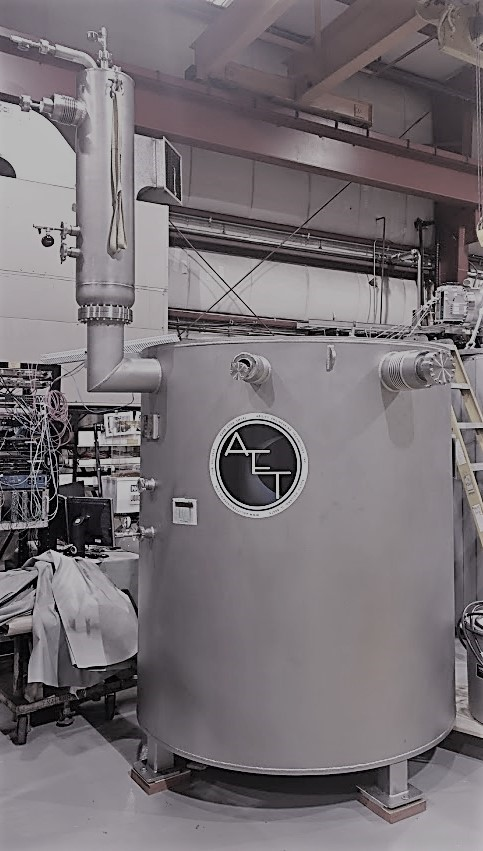
\includegraphics[width=0.3\linewidth]{sp-tpcelec-ICEBERG-cryostat.jpg}
  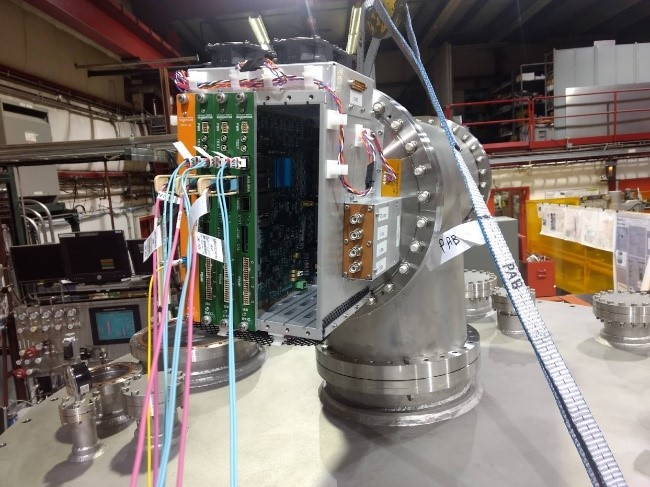
\includegraphics[width=0.6\linewidth]{sp-tpcelec-ICEBERG-Tee.jpg}
\end{dunefigure}

\begin{dunefigure}
	[\dword{iceberg} TPC and DAQ rack]
  {fig:ICEBERG-tpcdaq}
	{\dword{iceberg} TPC (left) and DAQ rack (right).}
  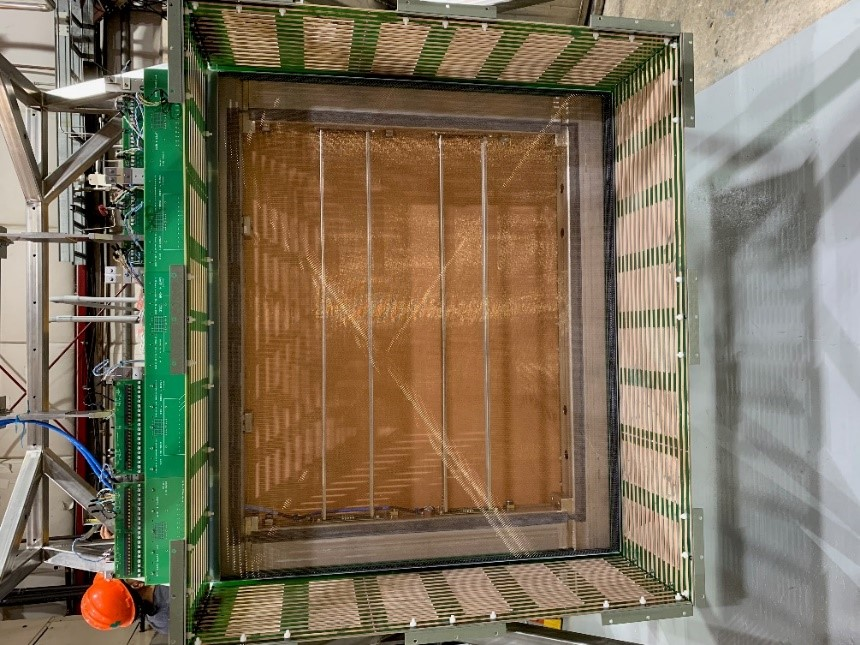
\includegraphics[angle=270,width=0.45\linewidth]{sp-tpcelec-ICEBERG-TPC.jpg}
  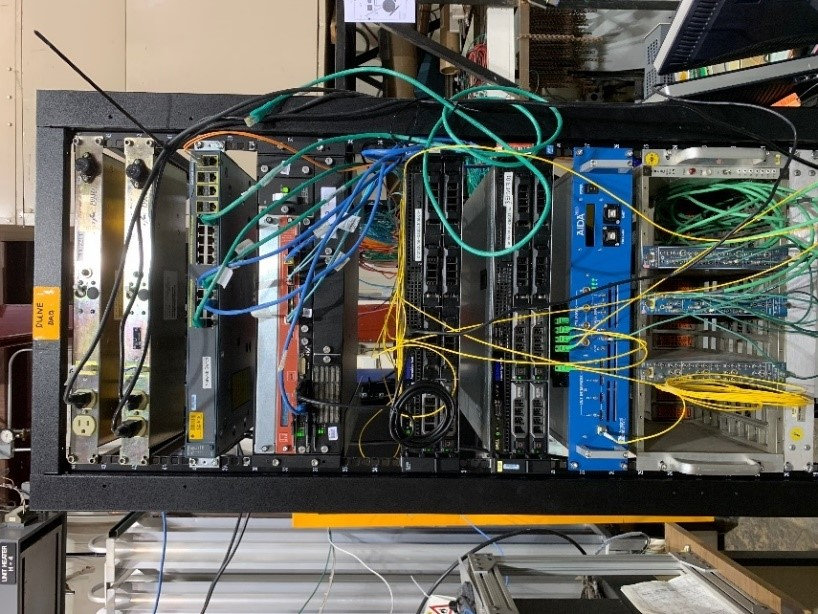
\includegraphics[angle=270,width=0.4\linewidth]{sp-tpcelec-ICEBERG-DAQ.jpg}
\end{dunefigure}

The \dword{fc} for the \dword{tpc} is constructed using printed circuit boards and is 
designed to provide 25 cm of drift space on both sides of the \dword{apa}. The cathode 
plane is made of a printed circuit board coated with copper and will be powered with 
-15~kV DC power. There is a 1 G$\Omega$ resistance between the strips of the \dword{fc}
creating a gradient field changing from -15~kV at the cathode to -1~kV near the 
\dword{apa}. The two sides of the \dwords{fc} cages are terminated on the \dword{apa}
ground with 156~M$\Omega$ resistors. 

The DUNE Cold Electronics is interfaced with the \dword{apa} using the printed circuit board on the top of the \dword{apa}.

The \dword{iceberg} power system that would power the detector, electronics, DAQ and cryogenics controls has been designed with an extreme care to isolate the detector and building grounds. A new 480 Volts transformer has been installed at the Proton Assembly Building to provide detector power for the TPC and the Cold Electronics. The impedance is continuously monitored by a ZMON rack. 

The distribution panel, which is at detector ground provides 208 and 120 volts power for the COLD Electronics Rack, which provides power to both the Cold Electronics and TPC in the cryostat through the Warm Interface Board and Power Points located in the Tee (see Figure~\ref{fig:ICEBERG-cryotee}). The MPOD in CE Power Rack provides -665, -370, 0 and 820 Volts to Grid, U, V and X planes respectively. It also provides -15 k Volts to the cathode plane. The Wiener PL506 provides 18, 48, 12 and -12 volts to the Power and Timing Card (PTC) located in the Tee at the top of the cryostat. These voltages are distributed to FEMB through the Warm Interface Board through the back plane of the crate.

The Data Acquisition (DAQ) System for the \dword{iceberg} consists of several subsystem currently being utilized at the ProtoDUNE at CERN.

The system is modular and could be upgraded to follow the overall DUNE DAQ development. The core of the DAQ system consists of two Scientific LINUX CPUs which communicates over 10 Gbps optical fiber links to Cluster on Board (COB). COB collects raw data from the Cold Electronics Warm Interface Board (WIB) over fiber and packages them for analysis by artDAQ running of the UNIX CPU. A pair of scintillators located at the top and bottom of the cryostat generates a cosmic trigger for the DAQ  using a Trigger Logic Unit (TLU).

The \dword{iceberg} will be primarily used for the development of the DUNE Cold Electronics. The initial system to establish a baseline for future comparison and development closely resembles the DUNE CE installed in ProtoDUNE at CERN. It consists of a 128 channels Front-End Mother Board, which is enclosed in a RF Box and connected with a Power and Signal cables to Warm Interface Board. The Warm Interface Board is located in a crate inside the Tee (Fig 1 (b)) and is powered using a Power and Timing Card.

In the 1st run of the cryostat we will establish the baseline performance of the DUNE Cold Electronics. Studies will be carried out to understand noise in the electronics and measures to reduce them. A new FEMB is under design by the collaboration. All the FEMB will be replaced with new electronics and studies will be performed to verify that the new design meets the DUNE requirements. The facility could be utilized for QA/QC if the electronics before installing them in the Far Detector.

%%%%%%%%%%%%%%%%%%
\subsubsection{Additional Test Facilities}
\label{sec:fdsp-tpcelec-qa-facilities-additional}

For \dword{ce} development, testing single prototypes at both room and cryogenic temperature is the first 
step, as many problems can be identified quickly without a full or partial TPC wire readout. A test dewar 
design developed by Michigan State University, referred to as the Cryogenic Test System (\dword{cts}), allows for
testing of the \dwords{femb} and \dwords{asic} at both room temperature and submerged in LN$_2$. Several
\dword{cts} were deployed at BNL for the \dword{pdsp} production \dword{femb} QC and SBND \dword{asic} QC. Several
others have already been deployed as Fermilab and other institutions to test further prototype \dword{femb}.
The \dword{cts} cooling process avoids the condensation of water from air that can otherwise interfere with the 
tests or damage the test equipment; two \dword{cts} units in operation at BNL are shown in Figure~\ref{fig:CTS}.

\begin{dunefigure}
[The Cryogenic Test System (\dword{cts})]
{fig:CTS}
{Cryogenic Test System: an insulated box is mounted on top of a commercial LN$_2$ dewar.  Simple controls allow the box to be purged with nitrogen gas and LN$_2$ to be moved from the dewar to the box and back to the dewar.}
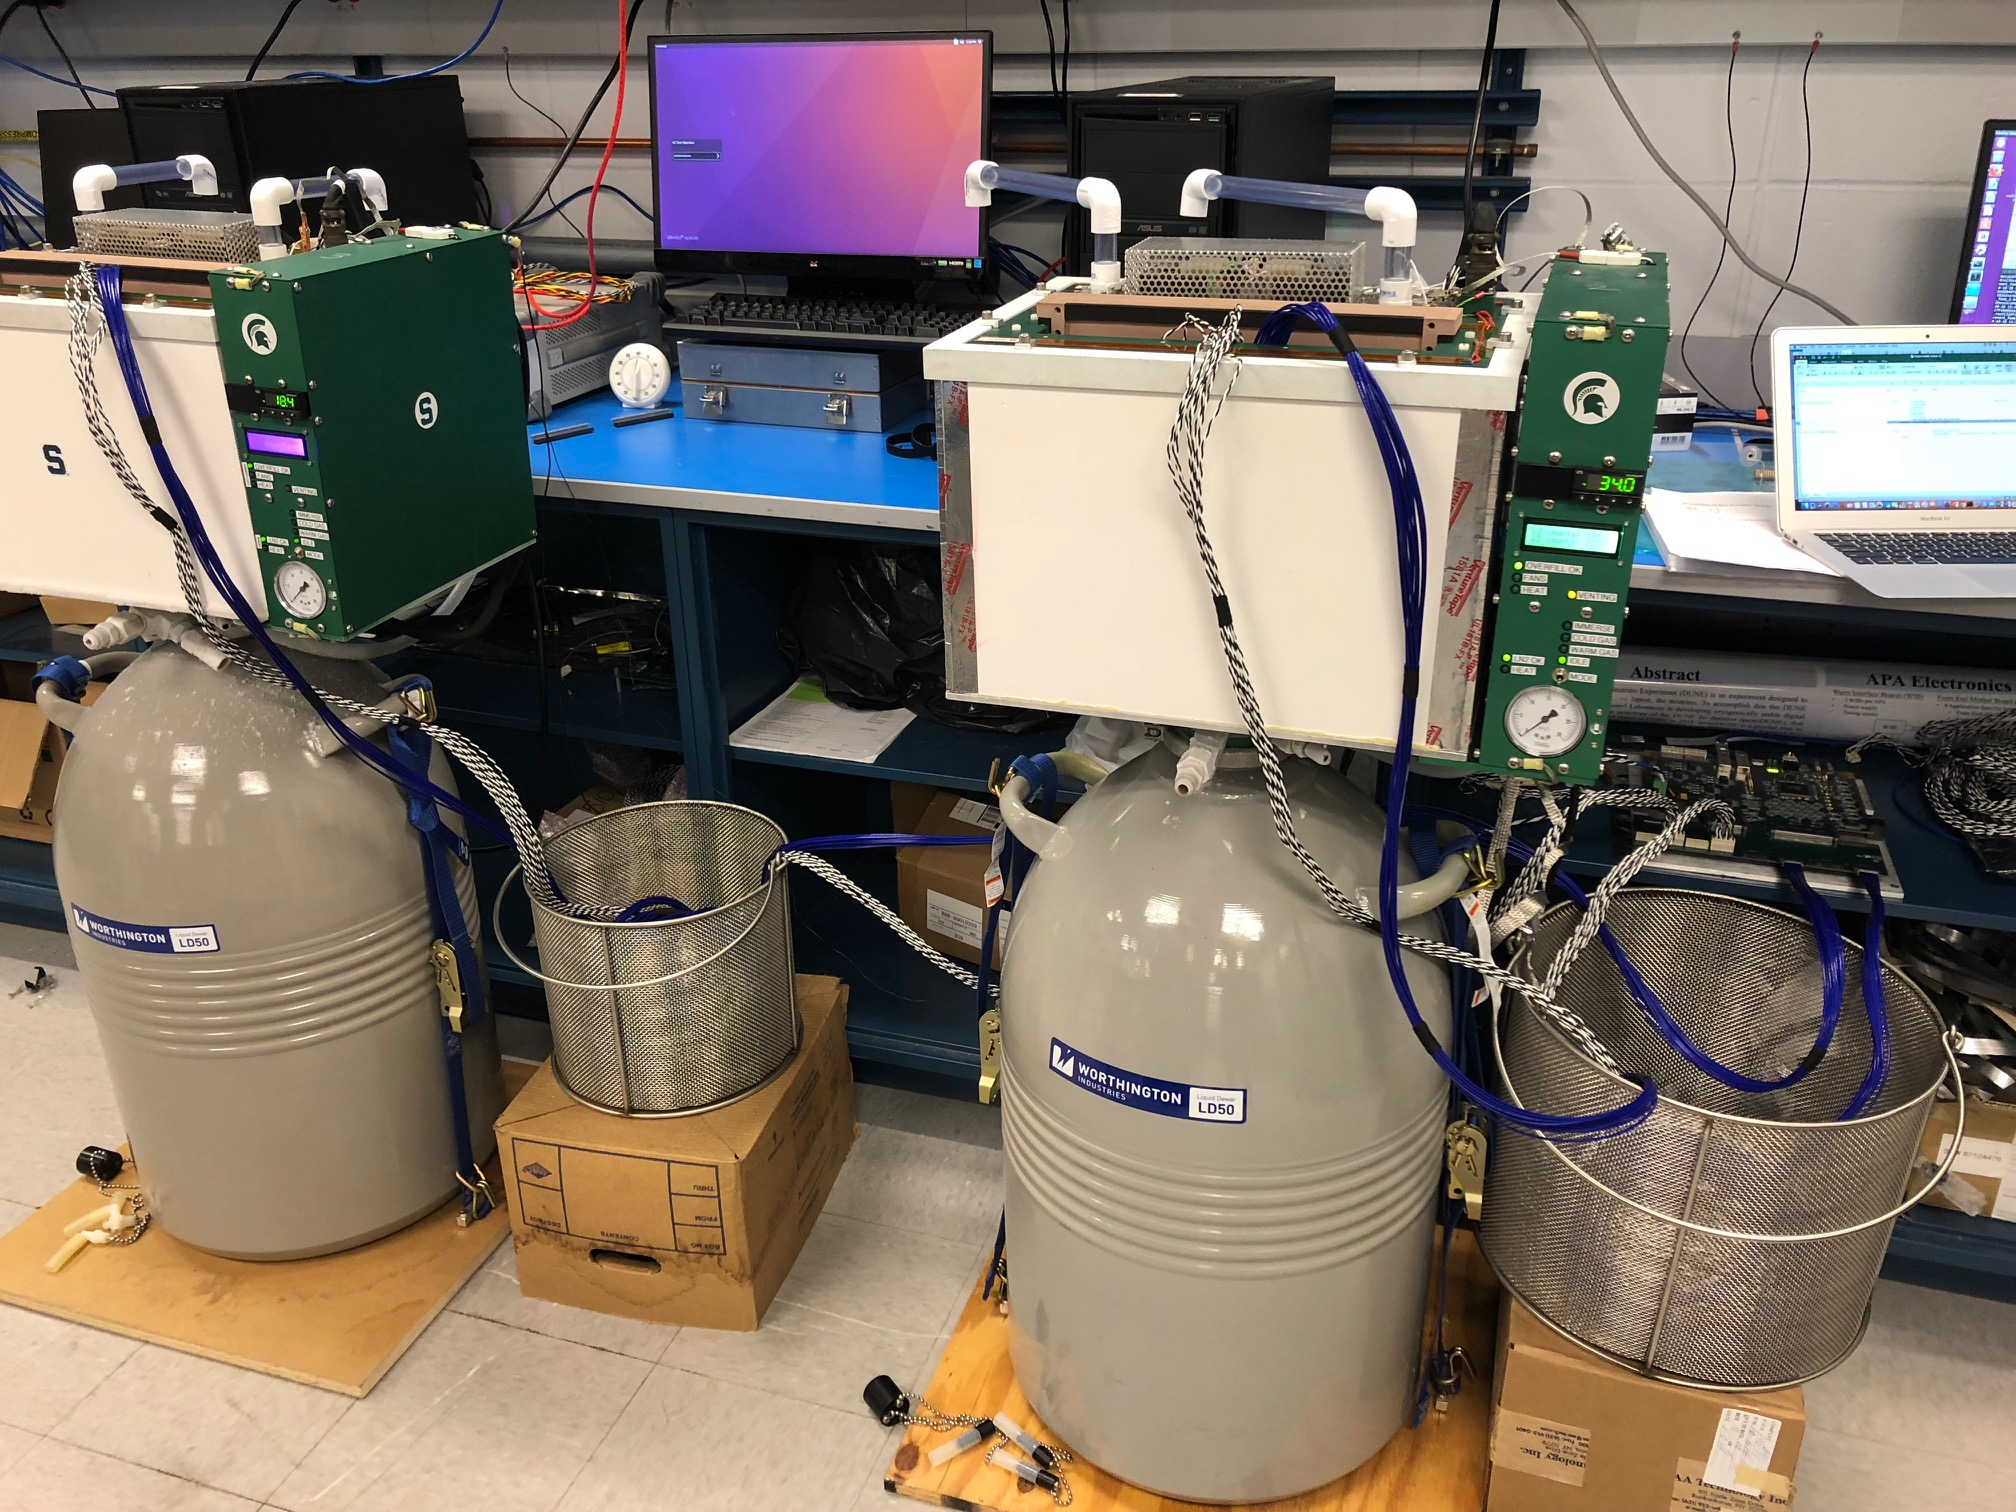
\includegraphics[width=0.4\linewidth]{sp-tpcelec-CTS2.jpeg}
\end{dunefigure}

Additionally, a quick access test stand with the \dword{femb} connected to an \dword{apa} inside a shielded 
environment that is in the same location as the \dword{femb} and \dword{asic} development is invaluable 
for rapid progress.  Two such facilities are available to DUNE: the ``\dword{iceberg}'' small TPC at \fnal and the 
\num{40}\,\% \dword{apa} test stand at BNL. \dword{iceberg} will be described in Section~\ref{iceberg-sux}.

The \num{40}\,\% \dword{apa} at BNL is a \SI{2.8}{m}~$\times$~\SI{1.0}{m} three-plane \dword{apa} with two 
layers of \num{576} wrapped ($U$ and $V$) wires and one layer of \num{448} straight ($X$) wires. It is read 
out by up to eight \dwords{femb} with the full \SI{7}{m} \dword{pdsp} length data and \dword{lv} power cables, 
four on the top and four on the bottom. The readout uses the full \dword{ce} system, with \dword{ce} flange 
and \dword{wiec}, as shown in Figure~\ref{fig:tpcelec_40apa}. Detailed integration tests of the \dword{pdsp}
\dword{ce} readout performance while following the DUNE grounding and shielding guidelines were done at the 
\num{40}\,\% \dword{apa}.

\begin{dunefigure}
[One side of the \num{40}\,\% \dword{apa} with four \dwords{femb} and the full \dword{ce} \fdth and flange.]
{fig:tpcelec_40apa}
{Left: one side of the \num{40}\,\% \dword{apa} with four \dwords{femb}.  Right: the full \dword{ce} \fdth and flange.}
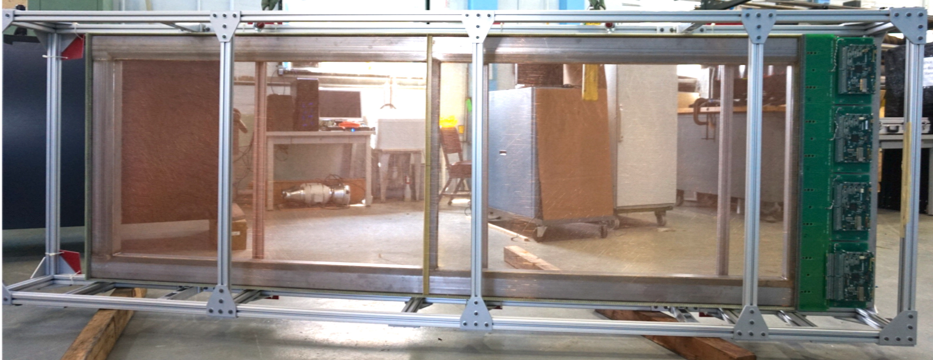
\includegraphics[width=0.72\linewidth]{sp-tpcelec-40-apa.png}
\hspace{3mm}
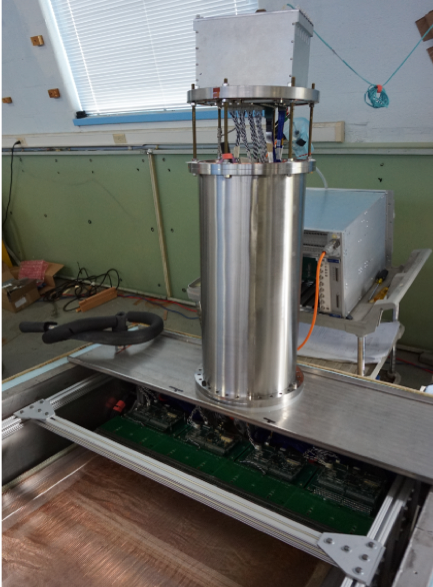
\includegraphics[width=0.2\linewidth]{sp-tpcelec-40-apa-ft.png}
\end{dunefigure}

%Additional input capacitance (equivalent to longer wire length) have been added to a subset of channels to project the \dword{enc} performance from the 40\% \dword{apa} teststand to the \dword{pdsp} and SBND detectors. The results from the \num{40}\,\% \dword{apa} indicate that, if the new \dword{adc} performs as expected, the full \dword{ce} system as installed on the test  stand at BNL will have a noise level in \lar around \num{500}\,e$^-$ and \num{600}\,e$^-$ for the collection and induction plane channels, respectively, in line with the CERN cold box tests described in Section~\ref{sec:fdsp-tpc-elec-qa-facilities-coldbox}.

%\begin{figure}
%    \centering
%    \includegraphics[width=0.9\linewidth]{tpcelec-40-apa-result.png}
%    \caption{\dword{enc} (in electrons) as a function of input capacitance (equivalent to input wire length) measured on the 40\% \dword{apa}. The \dword{enc} projections are based on the input wire length of the SBND and \dword{pdsp} detectors.}
%    \label{fig:tpcelec_40\dword{apa}_results}
%\end{figure}

Additionally, a Cold Box at CERN used in electronics tests for \dword{pdsp} is available for electronics testing 
in cold nitrogen gas. The advantage of the Cold Box is that it can cycle one full-size \dword{apa} with the full 
set of \num{20} \dword{femb} through gaseous nitrogen temperatures around \SI{150}{K} to validate the \dword{apa} 
performance as a complete \dword{ce} readout unit, as opposed to the 40\% \dword{apa} and \dword{iceberg} each of which have smaller
\dword{apa} footprints with fewer wires. The Cold Box is designed to be a Faraday cage, using the same grounding 
and shielding scheme that is implemented for the DUNE \single cryostat. It is read out by a complete \dword{ce} 
system for a single \dword{apa}, including a \dword{ce} flange and fully-loaded 
\dword{wiec} with five \dwords{wib} and one \dword{ptc}. Preliminary results from the \dword{pdsp} Cold Box testing 
for the second \dword{apa} installed at CERN are shown in Section~\ref{protodune-sux}.

%%%%%%%%%%%%%%%%%%%%%%%%%%%%%%%%%%%
\subsection{Reliability Studies}
\label{sec:fdsp-tpcelec-qa-reliability}

The TPC cold electronics system of the DUNE single phase far detector has to meet stringent requirements, such as low ($<<$ 1\%) failure rate of components installed on detector, inside the cryostat, without easy access during the \dunelifetime of detector operation. Reliability of all the components must be incorporated in the design and a dedicated analysis of all the possible failure mechanisms is required before finalizing the design of all \dwords{asic}, printed circuit boards, cables, connectors, and their supports, all of which are housed inside the DUNE far detector cryostat. 

There are a few HEP detectors that have been operated without intervention for a prolonged period of time, with limited losses of readout channels, and in extreme conditions like those of the DUNE cryostats:
\begin{itemize}
	\item NA48/NA64 liquid Krypton (LKr) calorimeter has 13,212 channels of JFET preamplifiers installed on detector. It has been kept at LKr temperature since 1998. The failure rate is $<$ 0.2\% for 20 years of operation so far.
	\item ATLAS liquid Argon (LAr) accordion EM Barrel (EMB) calorimeter has $\sim$110,000 readout signal channels, with up to seven connections and different circuit boards populated with resistor and diodes inside cryostat. The EMB calorimeter has been cold since 2004, for 14 years of operation.  So far the failure rate of readout channels is $\sim$0.02\%.
	\item ATLAS liquid Argon Hadronic Indict Calorimeter (HEC) has $\sim$5,600 readout channels through $\sim$35,000 cold preamplifier channels designed in GaAs technology on preamplifier and summing boards (PSB). The HEC cold electronics has been in cold operation since 2004, with $\sim$0.37\% failure rate during 14 years of operation. 
\end{itemize}
In addition, FERMI/GLAST is an example of a joint project between NASA and HEP groups that had a minimum mission requirement of five years and is on its way to achieving a stretch goal of ten years of operations in space. As the requirements can be rather different, it is important to examine and understand the various strategies for a space flight project compared to those of DUNE. Specifically launch "Shake and Bake" tests, redundancy requirements on critical infrastructure, and extensive test to failure, etc., may be inapplicable.

A preliminary list of reliability topics to be studied for the TPC electronics operated in LAr environment are:
\begin{itemize}
	\item The custom \dwords{asic} proposed for use in DUNE (\dword{larasic} + joint LBNL-FNAL-BNL ADC + \dword{coldata} \dword{asic}, or the SLAC \dword{cryo} \dword{asic}) incorporate design rules aimed at minimizing the hot carrier effect\cite{Li:2013ieee}\cite{Hoff:2015hax}, which is recognized as the main failure mechanism for integrated circuits operating at LAr temperature.
	\item For COTS components, accelerated lifetime testing, a standard test methodology used by the semiconductor industry, shall be devised to verify the expected lifetimes for operation in cryogenic temperature. A COTS ADC has undergone this procedure, to be qualified as a solution for the SBND experiment\cite{Chen:2018zic}.
	\item Print circuit board assemblies designed and fabricated to survive repeated immersions in LN$_2$.
	\item Capacitors operating voltage with sufficient margin, e.g. V$_{OP}<$ WVDC/2.
	\item Connectors and cables, usually major sources of detector channel failures, impose a testing challenge.
	\item A formal QA process for all TPC electronics components to be installed inside the cryostat.
\end{itemize}
The DUNE CE consortium has formed a working group tasked with studying reliability issues of these CE components and is preparing recommendations for the choice of \dwords{asic}, the design of printed circuit boards, and testing. This working group will review the segmentation of the cold electronics to understand which failures are going to have the largest impact on data taking; revisit recommendations for the \dword{asic} design, beyond those aimed at minimizing the hot carrier effect; revisit the industry and NASA standards for the design and fabrication of printed circuit boards, connectors, and cables, and make recommendations for the QA/QC procedures to be adopted during the fabrication of the cold electronics components. And in the review of the system aspects, to understand where it is desirable, necessary, and feasible to implement redundancy in the system, to minimize data losses due to single component failures. Later this working group will develop the QC program for the CE detector components, based upon experience from the ProtoDUNE-SP project.
